\subsection{Realizar Restore en Windows}

Primero, creamos tres archivos de texto que serán los objetos de nuestro backup y posterior restauración.

\begin{figure}[H]
    \centering
    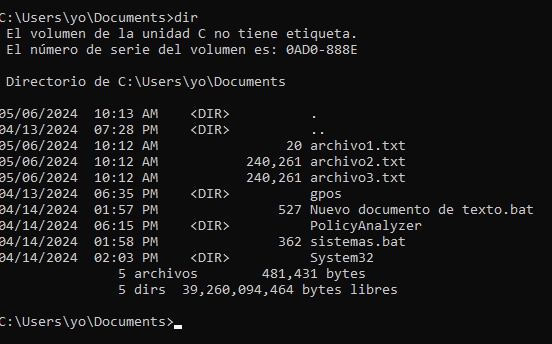
\includegraphics[width=0.5\linewidth]{instalacionBacula/archivosWin.png}
    \caption{Archivos originales creados en el directorio de documentos de Windows.}
\end{figure}

Procedemos a realizar el backup de estos archivos:

\begin{figure}[H]
    \centering
    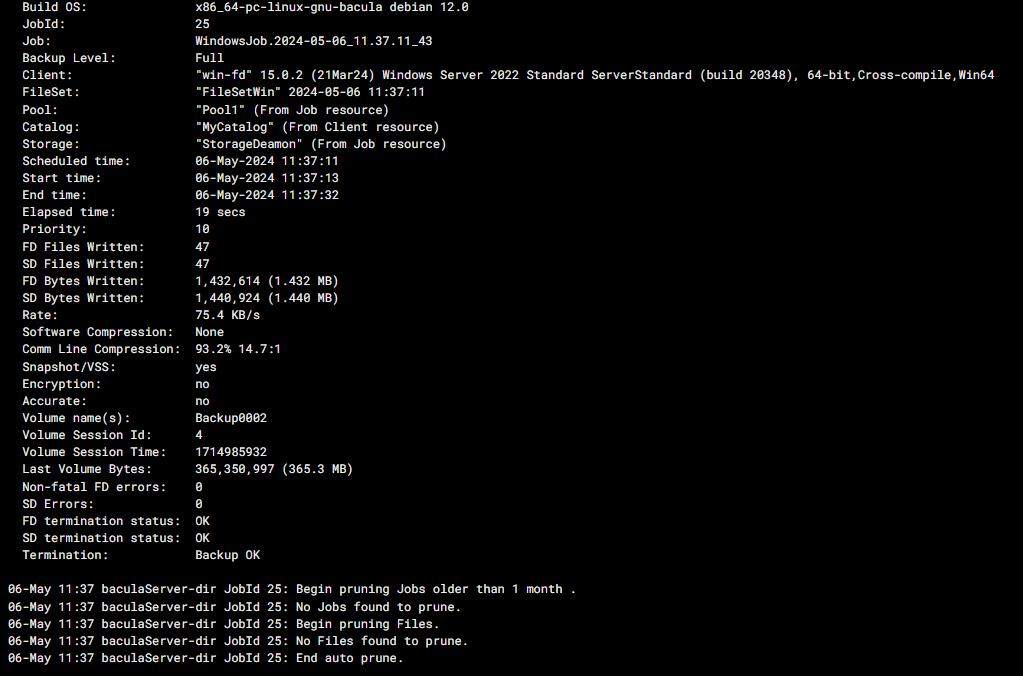
\includegraphics[width=0.5\linewidth]{instalacionBacula/backupWindows.png}
    \caption{Proceso de backup de los archivos mediante Bacula.}
\end{figure}

Después del backup, eliminamos los archivos 1 y 2 para simular una pérdida de datos y demostrar la capacidad de restauración:

\begin{figure}[H]
    \centering
    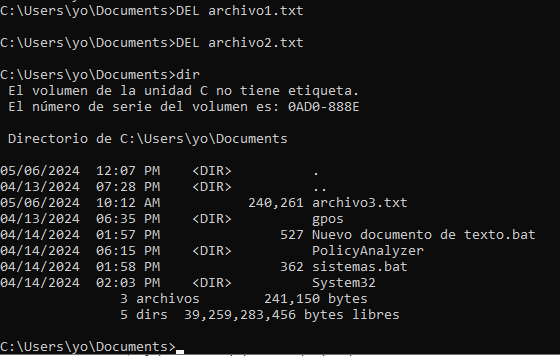
\includegraphics[width=0.5\linewidth]{instalacionBacula/borrarArchivosWin.png}
    \caption{Eliminación de archivos para simular pérdida de datos.}
\end{figure}

Realizamos la restauración de los archivos:

\begin{figure}[H]
    \centering
    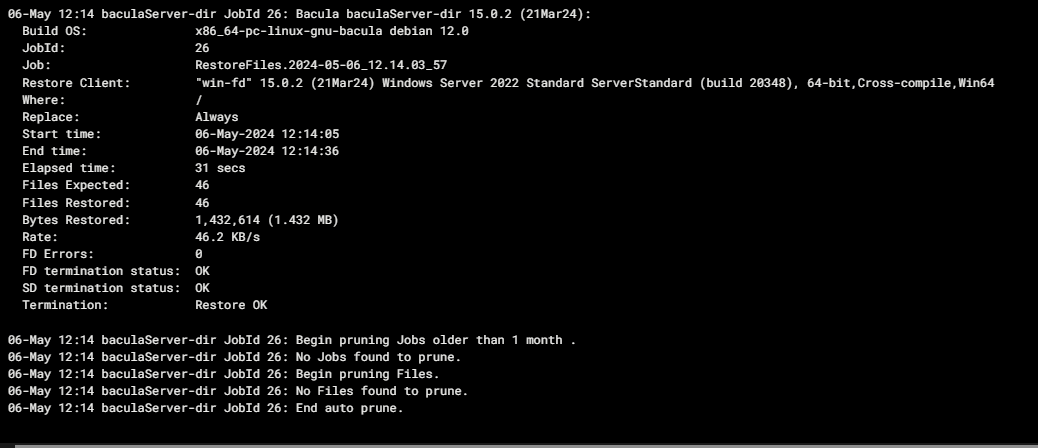
\includegraphics[width=0.5\linewidth]{instalacionBacula/restoreWIndows.png}
    \caption{Proceso de restauración de los archivos eliminados.}
\end{figure}

Confirmamos que los archivos han sido restaurados correctamente, como lo demuestra la siguiente vista del directorio:

\begin{figure}[H]
    \centering
    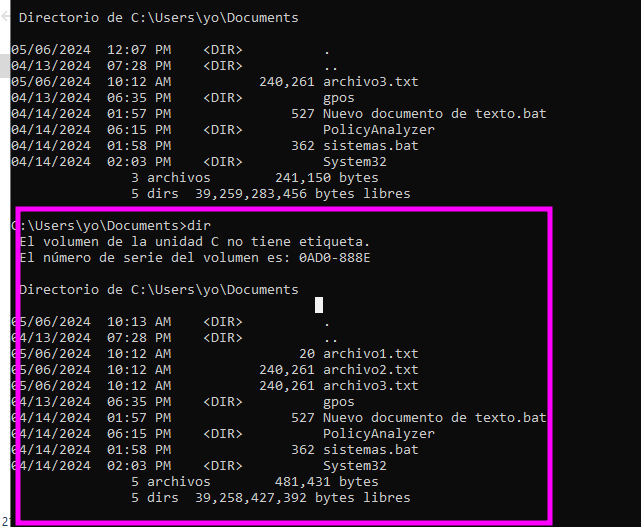
\includegraphics[width=0.5\linewidth]{instalacionBacula/restauracionWinCompleta.png}
    \caption{Archivos restaurados visualizados en el directorio de documentos.}
\end{figure}
